\section{Implementation and Prototypes}
\subsection{Rigid Prototype}
The first prototype was designed to test the capabilities of coils produced by the \textbf{HZDR research group}.
In the previous research done by the HZDR team, they tested the coil using a simple piece of \textbf{flexible magnetic tape} as a membrane and magnet.
This membrane is shaped like a "fish" so the tail can be fixed on a plane and the head can be free to bend up and down.
\begin{figure}[H]
    \centering
    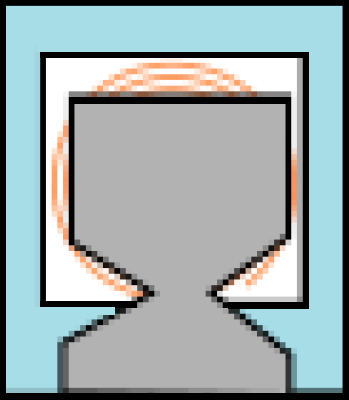
\includegraphics[width = 0.2\linewidth]{Figures/Dresden_test.png}
    \caption{Dresden coil HZDR test setup}
    \label{fig: Dresden_test}
\end{figure}
The pulp needed to be \textbf{suspended} at a certain distance to avoid pressing and stopping the membrane.

To solve this problem we developed a structure able to fulfill this requirement.
\begin{figure}[H]
    \centering
    \begin{subcaptiongroup}
      \centering
      \parbox[b]{0.2\textwidth}{
        \centering
        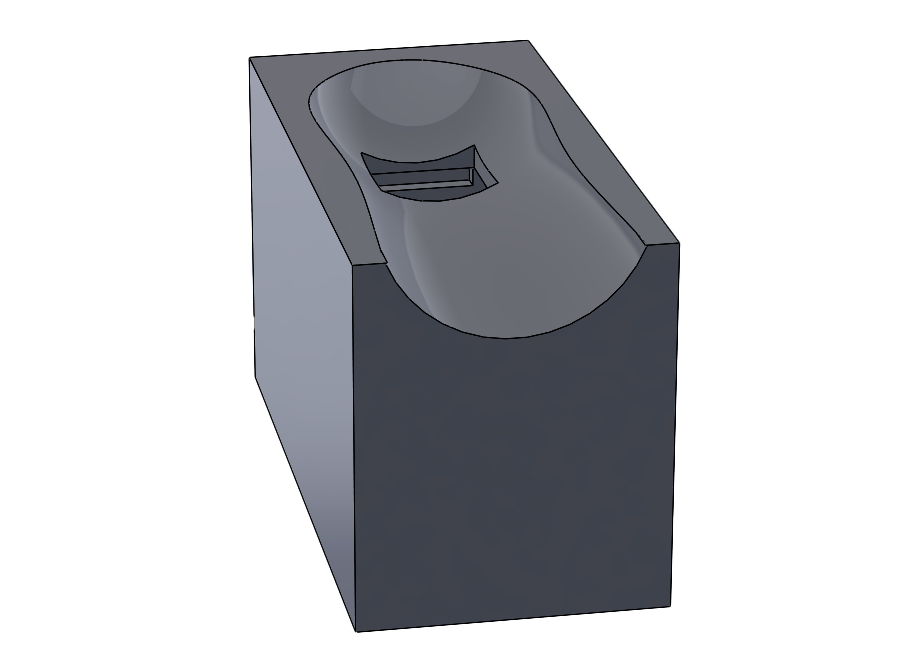
\includegraphics[width = 0.9\linewidth]{Figures/finger_holder.png}
        \caption{Finger resting surface}
      }
      \parbox[b]{0.2\textwidth}{
        \centering
        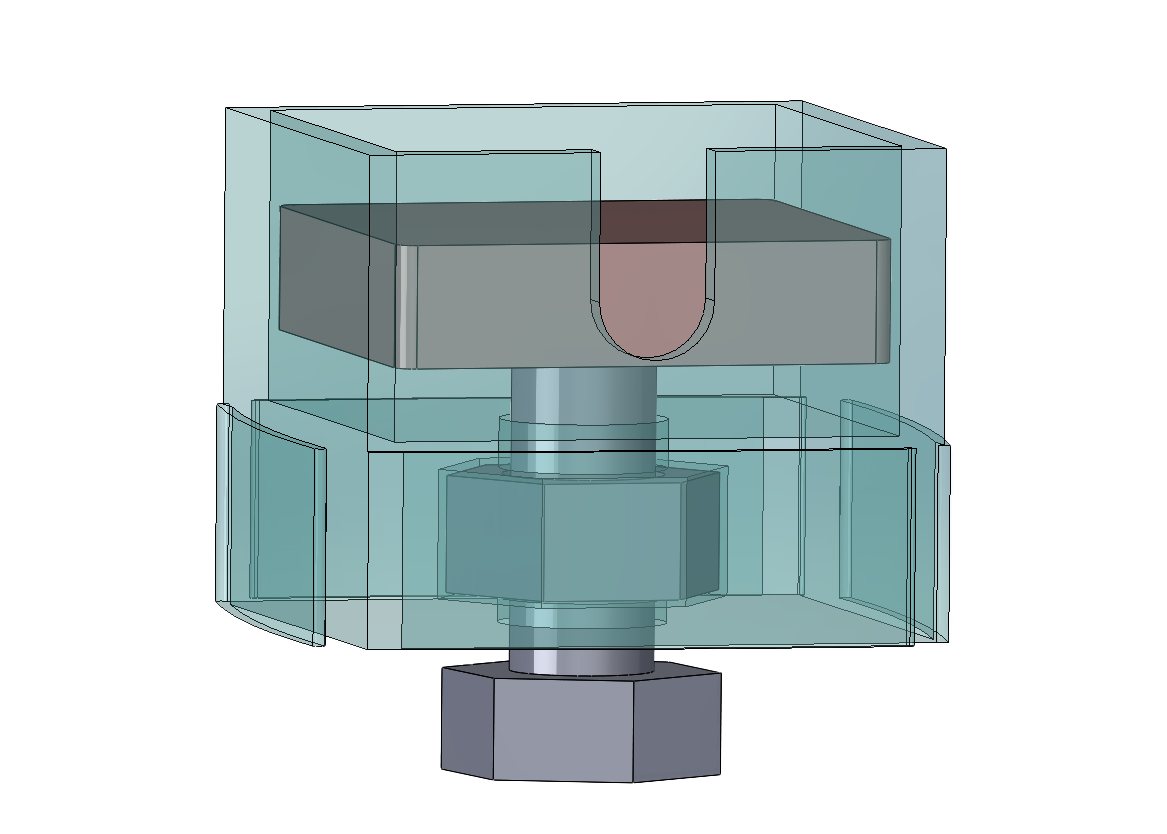
\includegraphics[width = 0.9\linewidth]{Figures/adj_platform.png}
        \caption{Finger platform}
      }
    \end{subcaptiongroup}
    \caption{Components of the first prototype}
\end{figure}
The coil and membrane are placed on top of the \textbf{height-adjustable platform}, to feel the vibrations the finger would lay on the hole of the resting surface.
We quickly moved on from this prototype as the coil was not able to generate \textbf{enough force} to be felt by the user because its \textbf{low power rating} limited its capability to generate a \textbf{strong enough magnetic field}.

\subsection{Wearable Rigid Prototype}
The following prototype was based on the flexible PCB coils. 
These have a \textbf{higher power rating}, can be \textbf{easily designed and manufactured} and are \textbf{sturdier} than the previous ones, especially under flexing conditions. 
A structure was designed to keep the coil in place and allow it to be \textbf{worn on the finger} through the use of silicon sleeves.
This sleeve was designed to be \textbf{adaptable to different finger sizes} and to \textbf{integrate a cylindrical magnet} on the pulp.
\begin{figure}[H]
    \centering
    \begin{subcaptiongroup}
        \centering
        \parbox[b]{0.2\textwidth}{
            \centering
            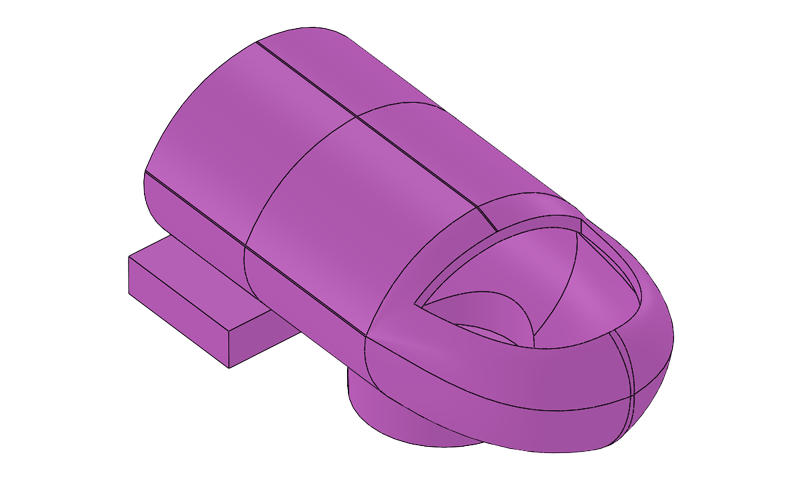
\includegraphics[width=0.2\textwidth]{Figures/silicon_sleeve_front.png}
        }
        \parbox[b]{0.2\textwidth}{
            \centering
            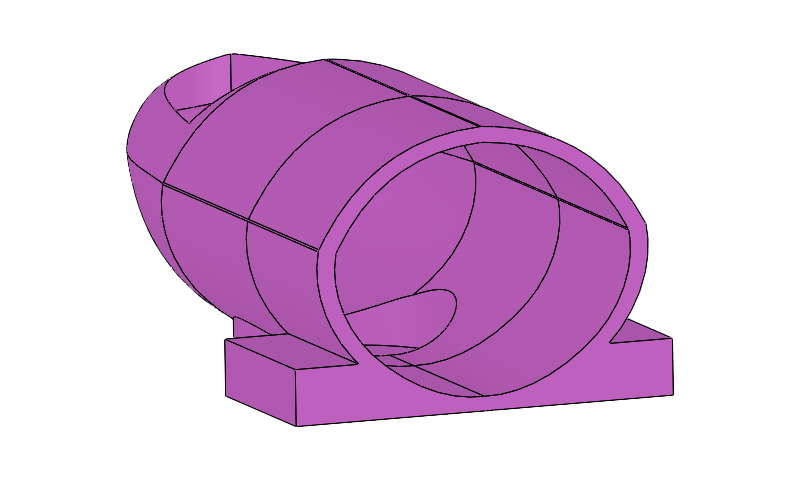
\includegraphics[width=0.2\textwidth]{Figures/silicon_sleeve_back.png}        
        }
    \end{subcaptiongroup}
    \caption{Finger silicon sleeve front and back view}
\end{figure}
The silicon sleeve could be then connected to the assembly where the coil and a heatsink were placed through its lateral mounting wings.
\begin{figure}[H]
    \centering
    \begin{subcaptiongroup}
        \centering
        \parbox[b]{0.2\textwidth}{
            \centering
            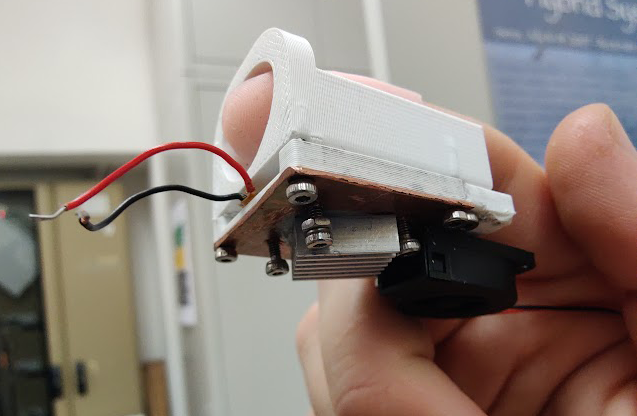
\includegraphics[width=0.2\textwidth]{Figures/rigid_prot_btm.png}
        }
        \parbox[b]{0.2\textwidth}{
            \centering
            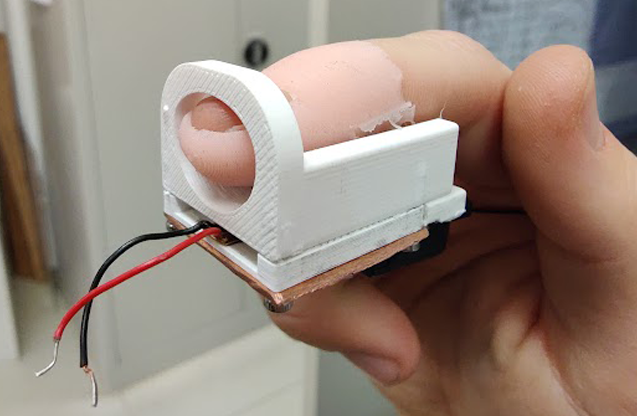
\includegraphics[width=0.2\textwidth]{Figures/rigid_prot_top.png}
        }
    \end{subcaptiongroup}
    \caption{Bottom and top view of the real prototype}
\end{figure}
This prototype showed \textbf{great improvements} over the previous one: the \textbf{magnet} was kept \textbf{at the right distance} from the coil and the vibrations were \textbf{much more noticeable}, and being wearable made it much easier to use.
Its biggest problem was the \textbf{silicon sleeve}, as the silicon tends to \textbf{absorb some of the vibrations} and the softness of the material made the mounting mechanism a bit \textbf{unreliable}.  
We also had to add a small blowing fan to the heatsink to keep the coil cool as it would \textbf{heat a lot} after a few minutes of use.

\subsection{Flexible Mat Prototypes}
The final prototype was designed to be a \textbf{flexible silicon mat where all components were integrated}, including the membrane.

\newsavebox{\largestimage}
\begin{figure}[H]
    \centering
    \savebox{\largestimage}{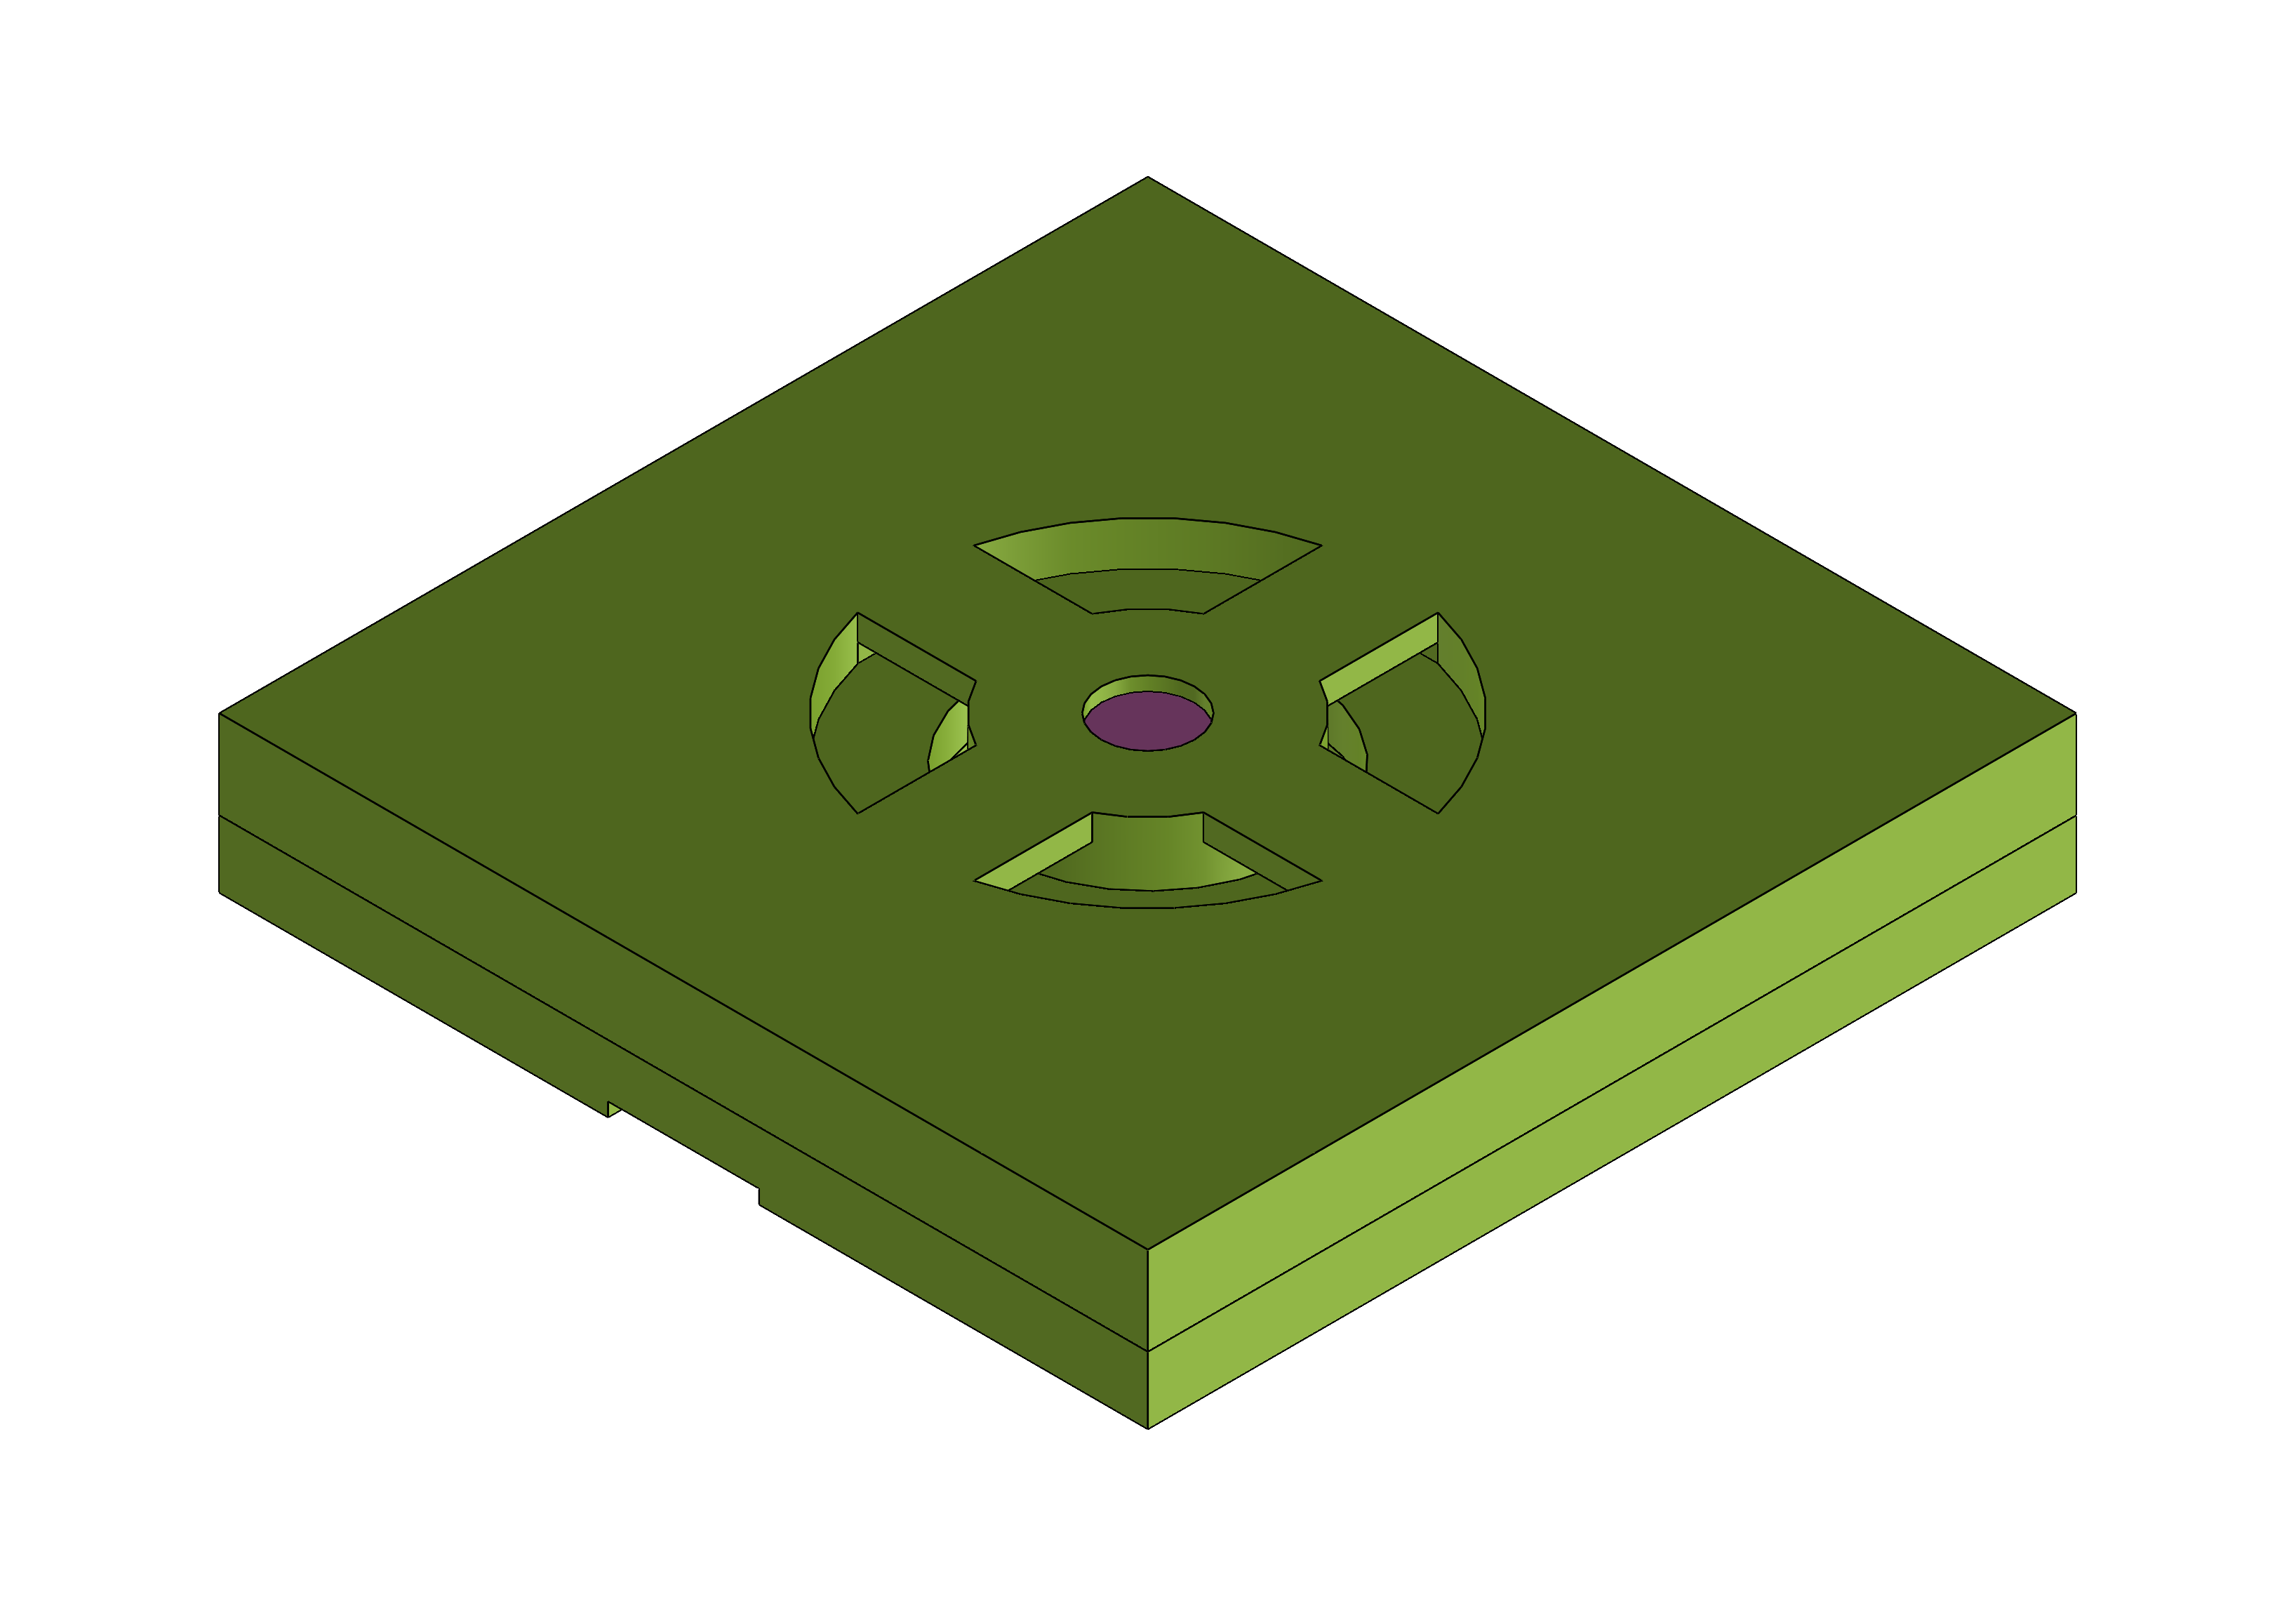
\includegraphics[width=0.2\textwidth]{Figures/membrane_v1.png}}
    \begin{subcaptiongroup}
        \centering
        \parbox[b]{0.2\textwidth}{
            \centering
            \usebox{
                \largestimage
            }
        }
        \parbox[b]{0.2\textwidth}{
            \centering
            \raisebox{\dimexpr.5\ht\largestimage-.5\height}{
                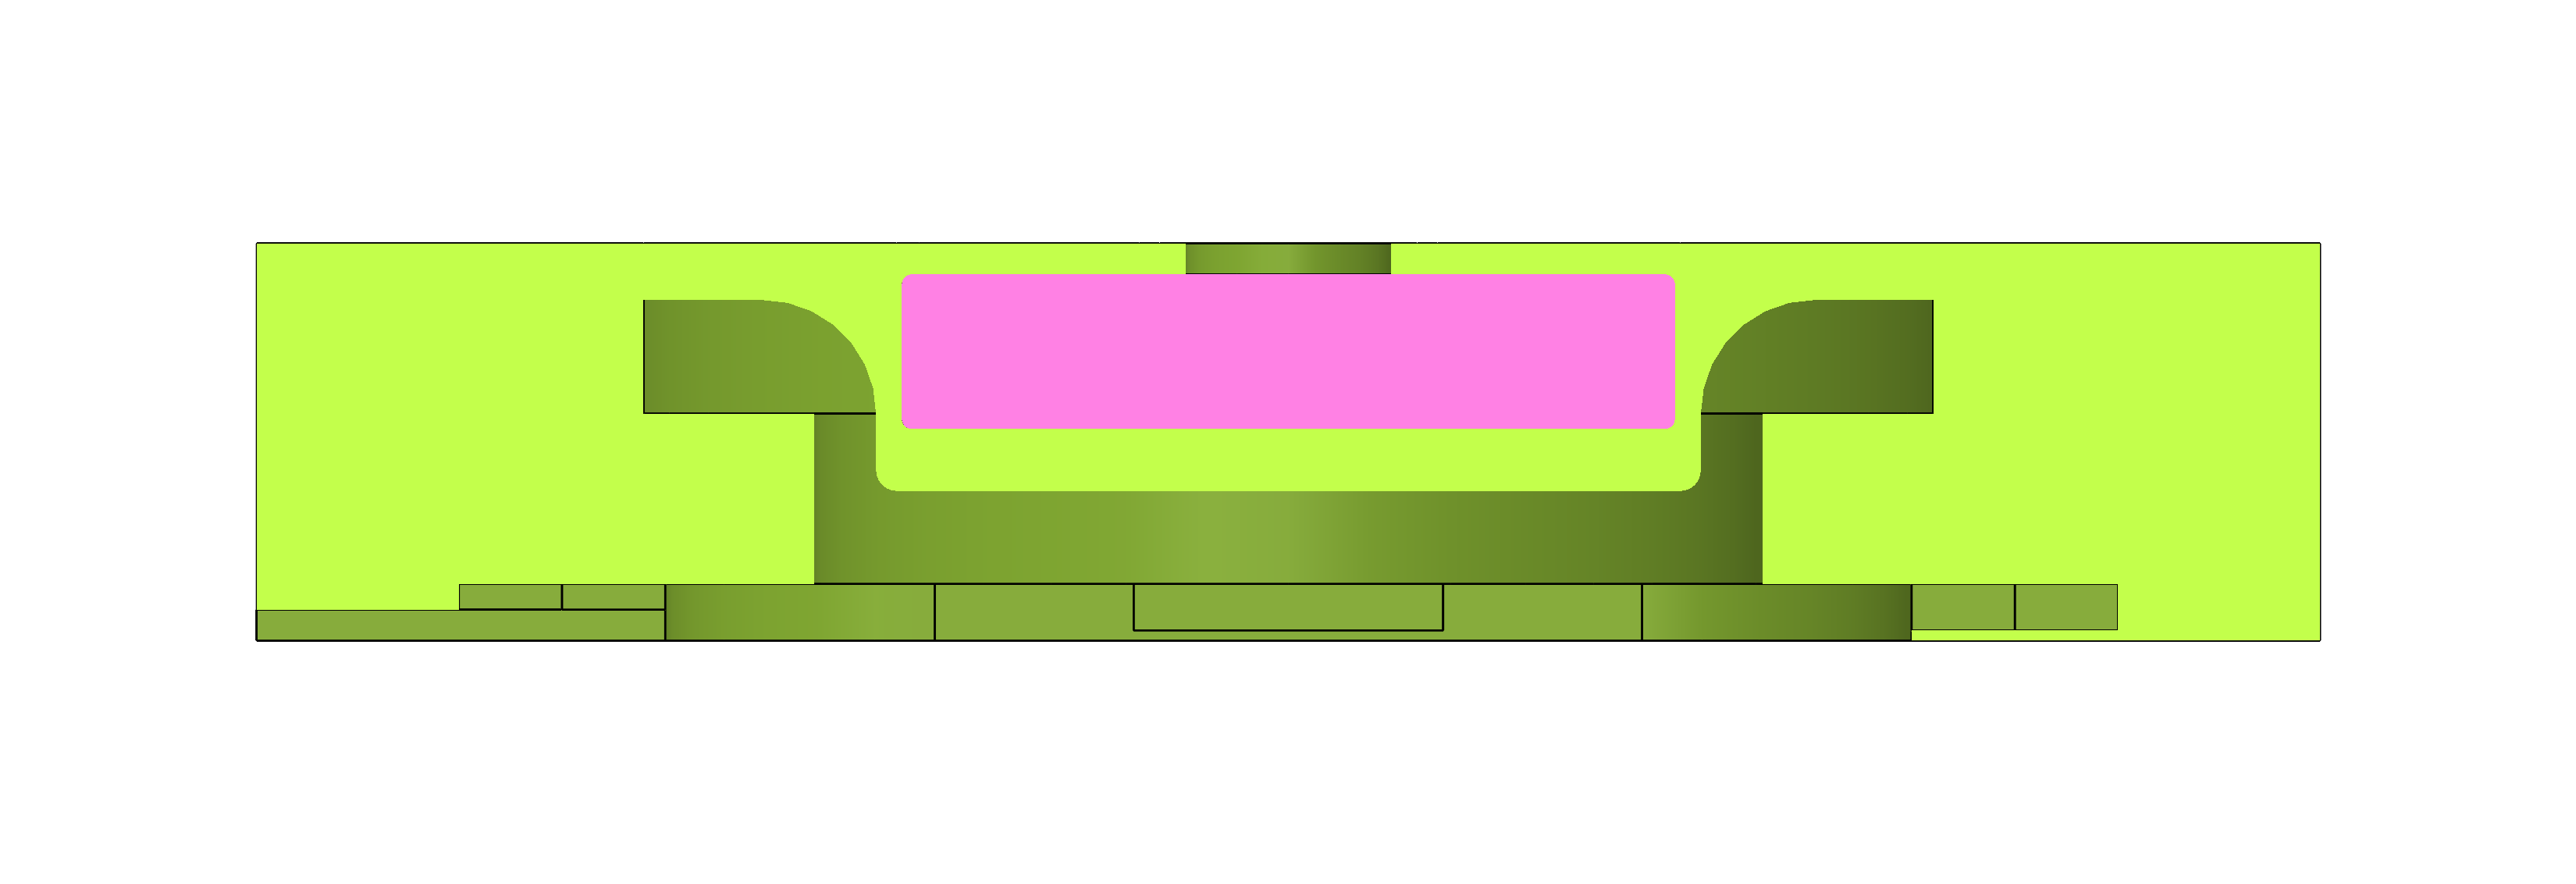
\includegraphics[width=0.2\textwidth]{Figures/membrane_v2_section.png}
            }
        }
    \end{subcaptiongroup}
    \caption{Top and section view of the flexible mat prototype}
\end{figure}
The magnet is suspended inside the silicon membrane and the coil is kept in place at the bottom of the mat.
The coil is kept inside the silicone structure thanks to a \textbf{flexible component} that is in part encased in the silicon and \textbf{acts as a trap}.

\newsavebox{\bigimage}
\begin{figure}[H]
    \centering
    \savebox{\bigimage}{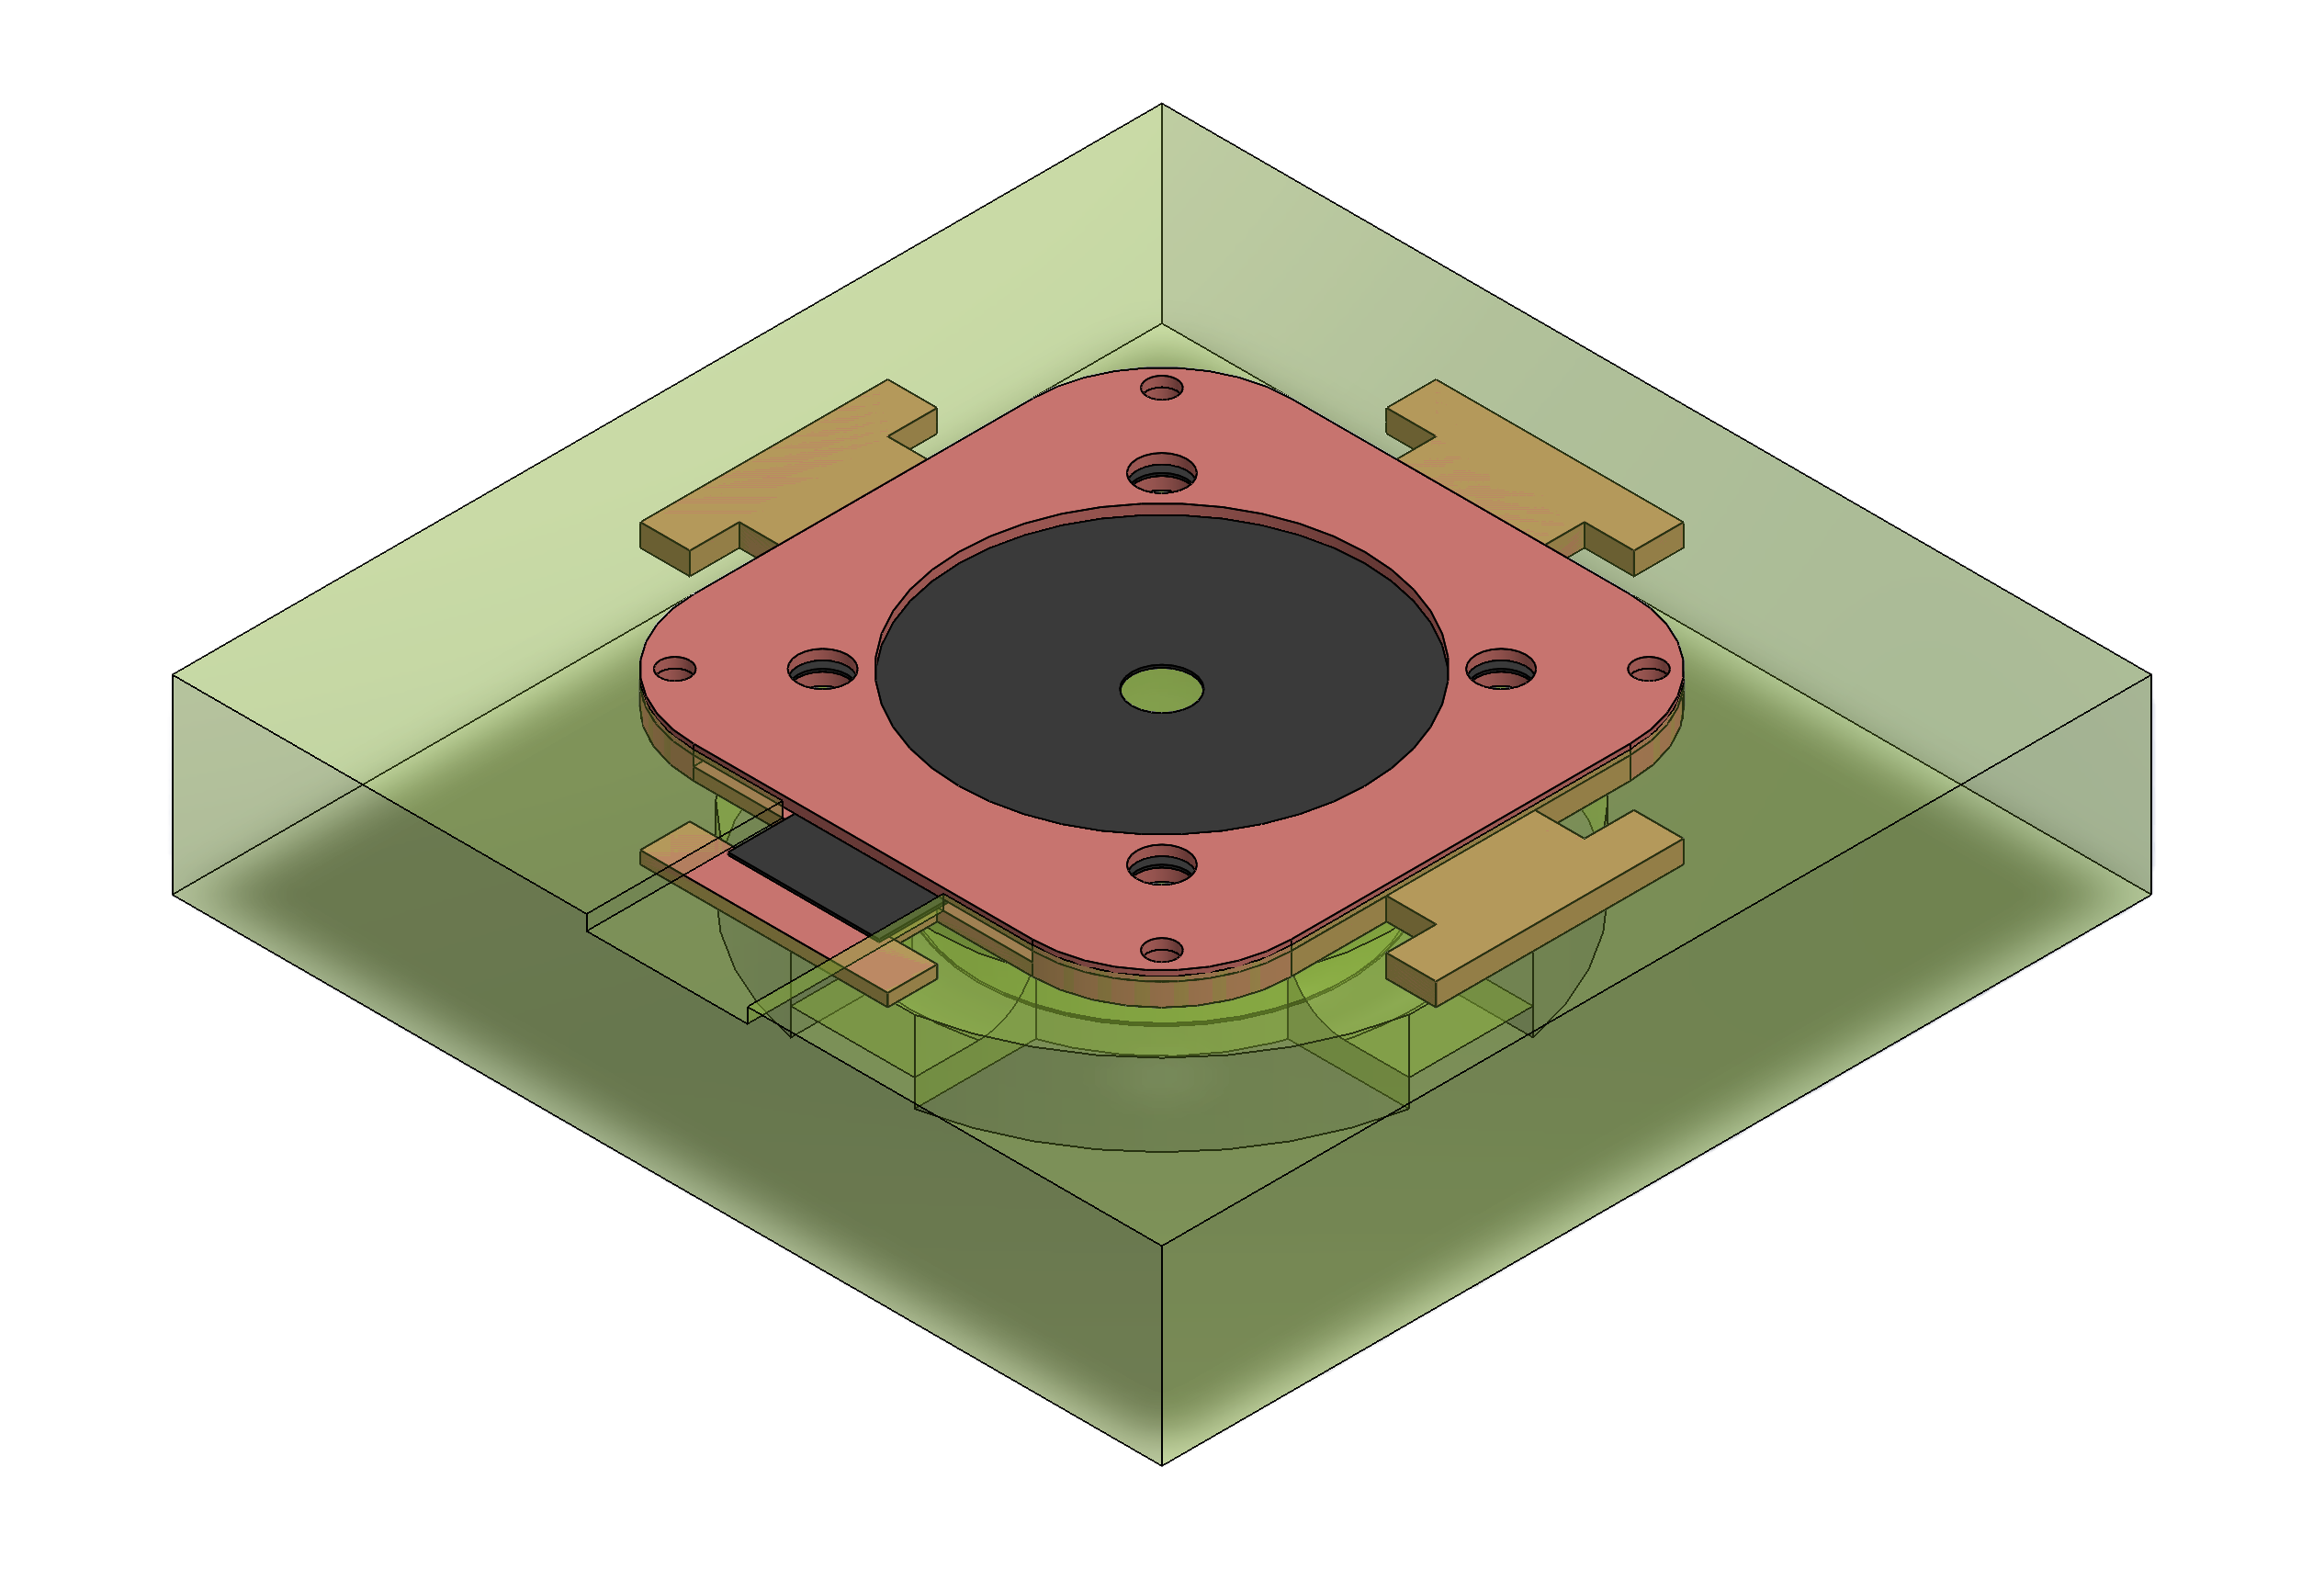
\includegraphics[width=0.2\textwidth]{Figures/coil_trap_in_mat.png}}
    \begin{subcaptiongroup}
        \centering
        \parbox[b]{0.2\textwidth}{
            \centering
            \raisebox{\dimexpr.5\ht\bigimage-.5\height}{
                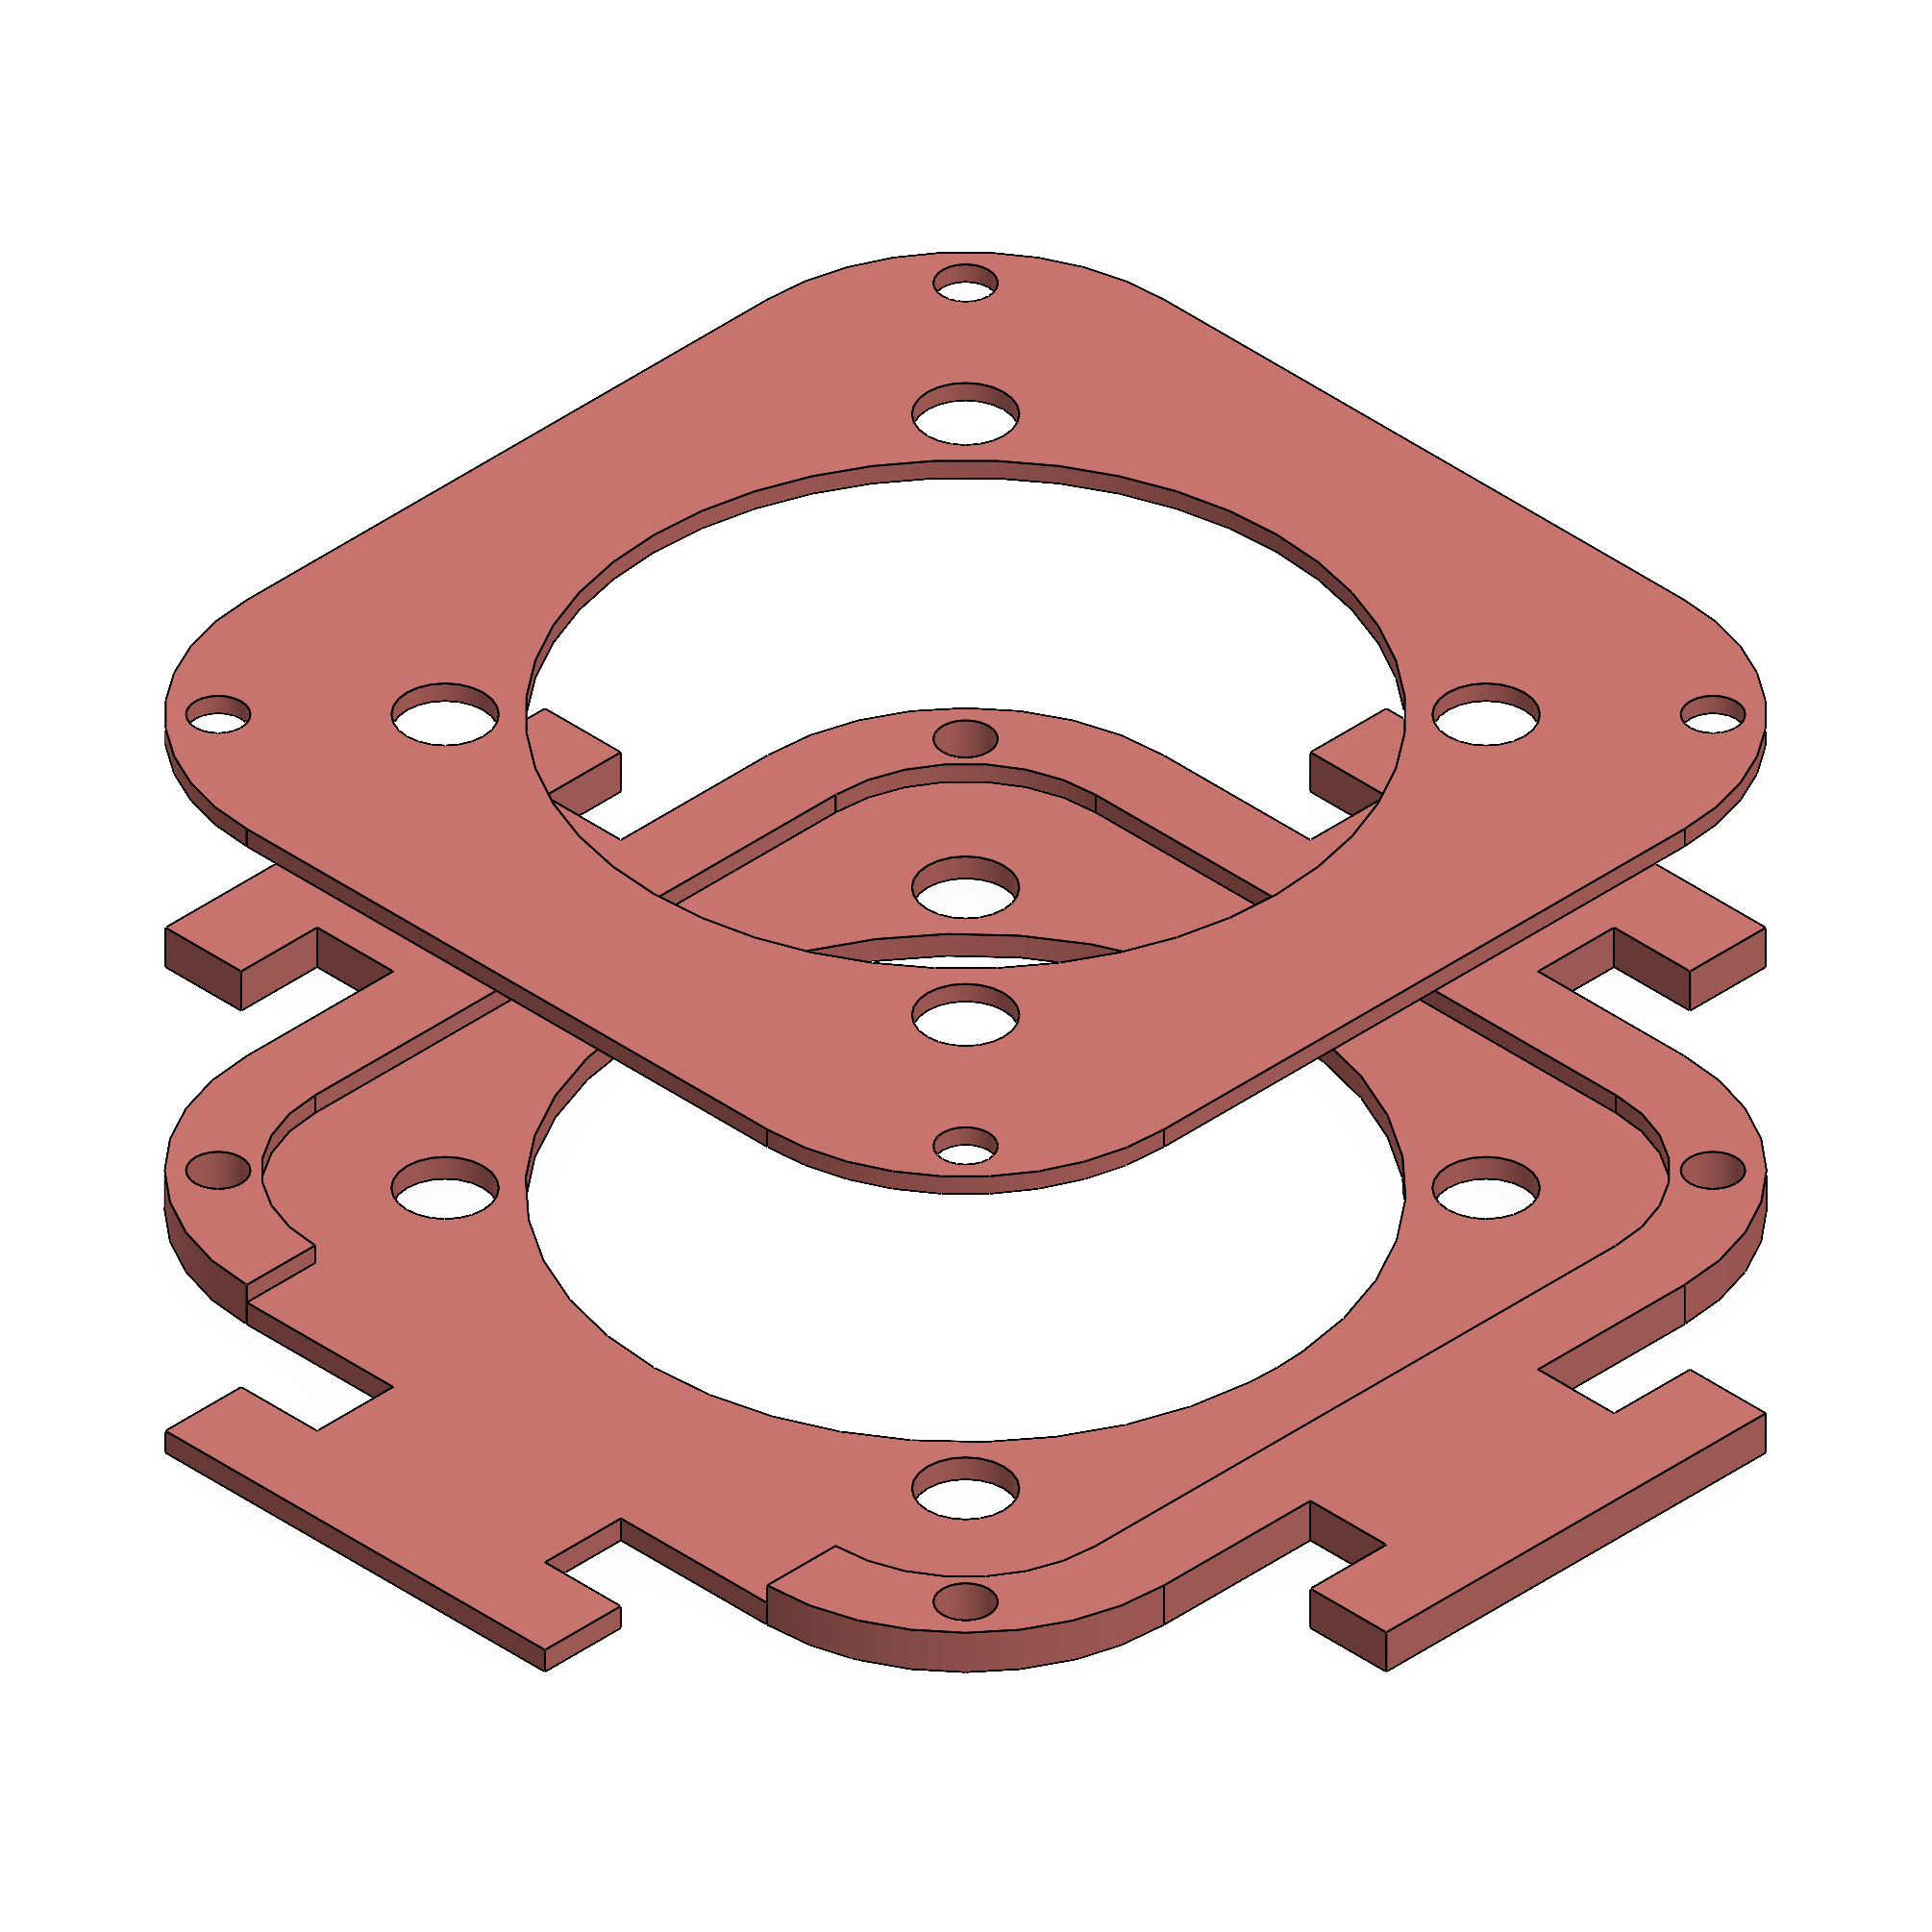
\includegraphics[width=0.15\textwidth]{Figures/coil_trap_expl.png}
            }
        }
        \parbox[b]{0.2\textwidth}{
            \centering
            \usebox{
                \bigimage
            }
        }
        
    \end{subcaptiongroup}
    \caption{Flexible coil trap.}
\end{figure}

This component allows the coil to be kept at an \textbf{optimal distance} from the magnet letting the membrane be \textbf{free to vibrate}.
This prototype resulted in the \textbf{best performance}: the vibrations were more noticeable, the mat was easy to interact with and the device could \textbf{easily flex}.
Nevertheless, we were \textbf{still not satisfied with the strength of the vibrations} it produced, the coil's problems with heating were still present and we had some \textbf{fragility problems} with the membrane and \textbf{flexing issues} with the coil trap. 

\subsection{Experimentation and Evaluation}
During our testing, we measured the \textbf{heating} production of the coil and the \textbf{force produced} by the last prototype membrane.
\subsubsection{Heating Testing}
We powered the coil with an input \textbf{voltage sweep both in DC and AC} conditions while measuring its surface temperature using a \textbf{thermocouple}. The limit of the sweep was chosen to be the maximum voltage that the coil could handle before reaching its \textbf{thermal runaway point}.
\begin{figure}[H]
    \centering
    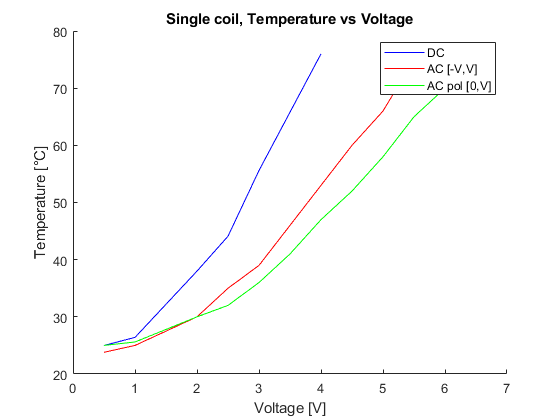
\includegraphics[width = 0.5\linewidth]{Figures/Temp_vs_Volt_1_coil.png}
    \caption{Temperature vs Voltage for one coil.}
    \label{fig: Single_coil_heating_tests}
\end{figure}
As we can observe in figure \ref{fig: Single_coil_heating_tests}, in AC conditions, especially for unipolar signals, the coil can sustain \textbf{higher voltages}; this is because sinusoidal signals have a \textbf{lower RMS} value than DC ones.

\subsubsection{Force Testing}
We measured the force produced by the membrane using an \textbf{ATI TW-Nano17 force sensor}. The prototype's coil was powered with a \textbf{heartbeat-like signal}, as it's a \textbf{very low RMS} signal that allows us to run the coil at \textbf{30V peak voltage}.
This was necessary because the sensor \textbf{sensitivity was too low} to measure the force produced by sinusoidal signals at \textbf{6V}.
\begin{figure}[H]
    \centering
    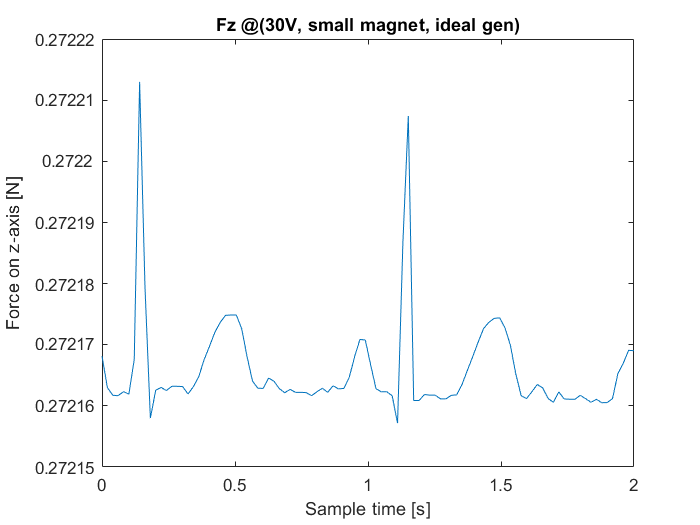
\includegraphics[width = 0.5\linewidth]{Figures/Fz_@30V_small_magn_idealgen.png}
    \caption{Force profile of the generated by the heartbeat signal.}
    \label{fig: Force_profile}
\end{figure}
From figure \ref{fig: Force_profile} we can observe that the membrane produces a \textbf{constant force of about 0.2N}, due to the silicone membrane itself, and the \textbf{net force} produced by the coil at the peak of the signal is in the order of \textbf{$5\cdot10^{-5}$N}.